\documentclass[main.tex]{subfiles}
%\usepackage{functions}
\begin{document}
%%%%%%%%%%%%%%%%%%%%%%%%%%%%%%%%%%%%
\pgfkeys{/pgf/fpu=true}
%%%%%%%%%%%%%%%%%%%%%%%%%%%%%%%%%%%% Define Constant for pgf
%\pgfmathparse{} %
%\edef\Gconst{\pgfmathresult}

\chapter{Esperienza 3: condizione di risonanza}

\section{Schema dell'esperienza}

\subsection{Materiali}
%decodearray={0.2 0.5},
\begin{wrapfigure}[20]{r}{0.3\textwidth} 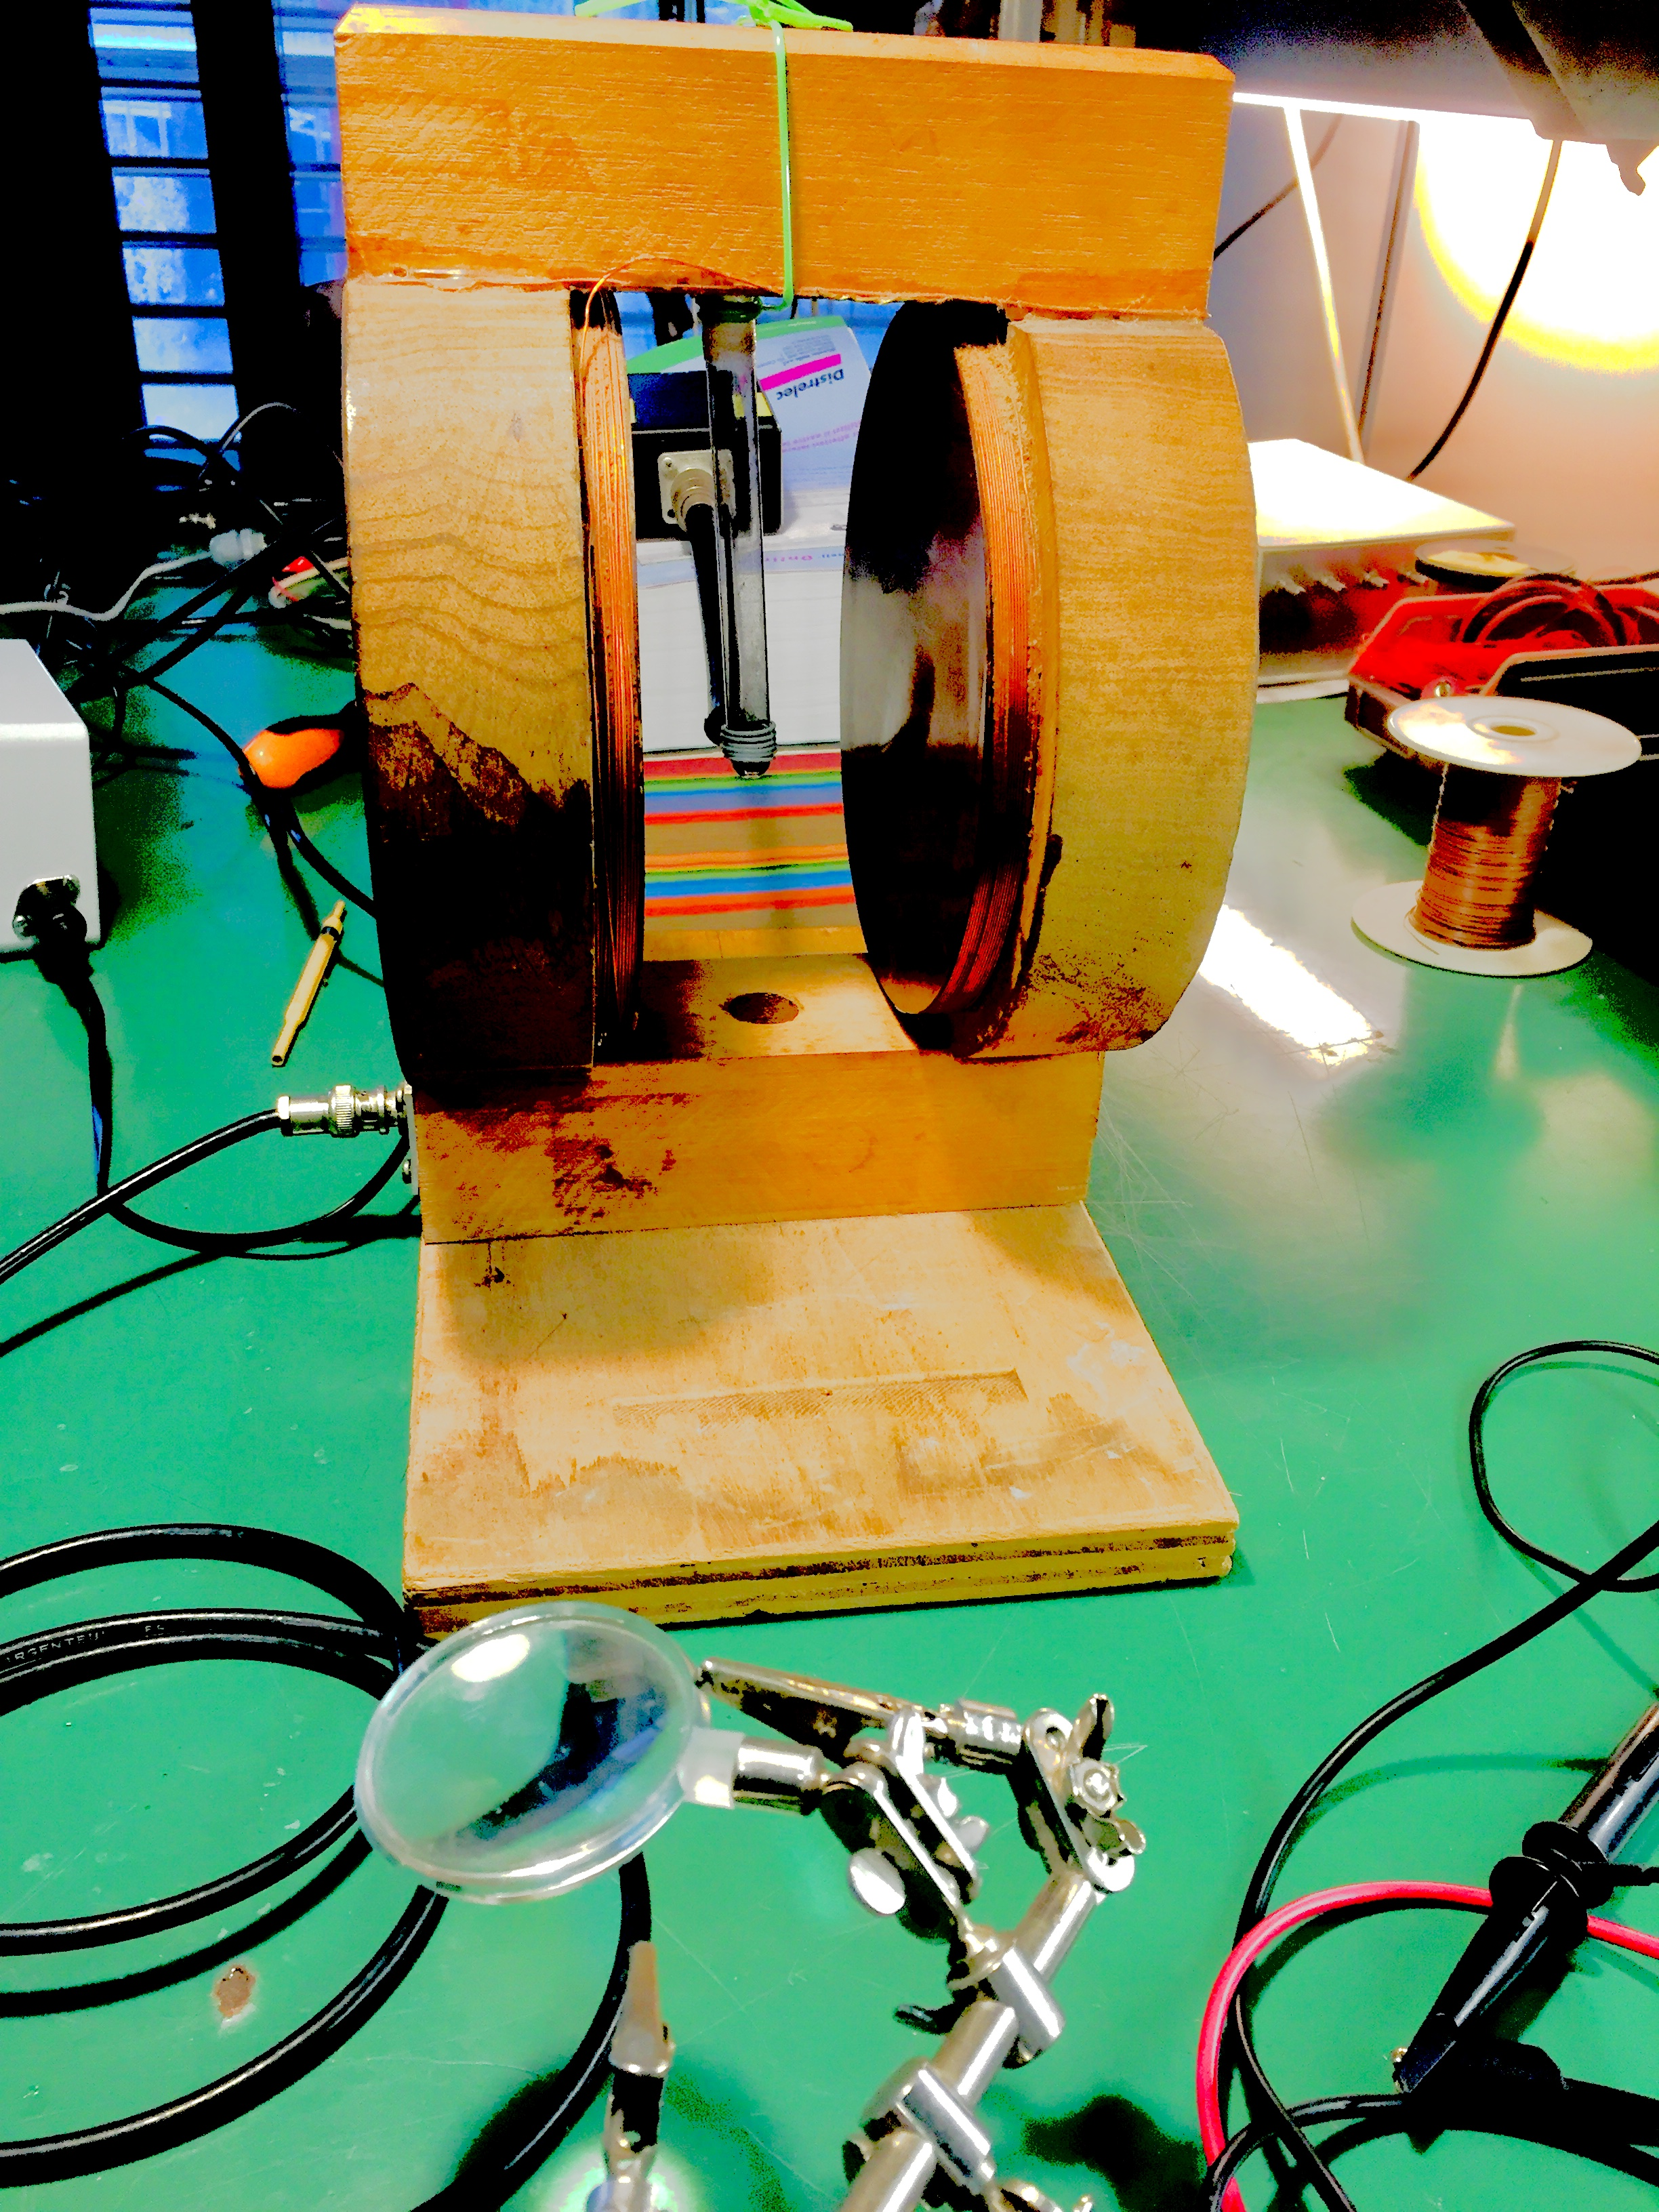
\includegraphics[trim={0cm 0 0 0},clip, width=0.3\textwidth]{B0resonance}\label{fig:B0resonance} \end{wrapfigure}

Il campione \'e inserito nella bobina in cui passa corrente AC con frequenza tra \SIrange{12}{22}{\mega\hertz} e immerso nel campo magnetico statico generato dal magnete DC: \SIrange{6}{8}{\gauss} per corrente \SIrange{180}{200}{\milli\ampere}. Inoltre un rivelatore di picco \'e usato per determinare la caduta di tensione ai capi del circuito AC.

\subsection{Procedimento}

Si varia la corrente nella bobina DC, quindi il campo magnetico generato dalla bobina.

\edef\frequno{20e6}    %RF freq uno
\edef\freqdue{16.9e6}    %RF freq due
\edef\Iuno{200e-3}    %corrente minimo corrente di picco uno
\edef\Idue{170e-3}    %corrente minimo corrente di picco due

Le correnti che corrispondono a minimo della corrente di picco sono \SI{200}{\milli\ampere} e \SI{170}{\milli\ampere} per rispettivamente corrente nella bobina a RF di \SI{20}{\mega\hertz} e \SI{16.9}{\mega\hertz}. 

Verifichiamo che esiste relazione lineare tra frequenza del campo oscillante e campo magnetico statico, proporzionale alle corrente, alla risonanza ($\nu_{ris}/I\propto\pgfmathparse{\frequno/\Iuno}\pgfmathprintnumber{\pgfmathresult}$, $\nu_{ris}/I\propto\pgfmathparse{\freqdue/\Idue}\pgfmathprintnumber{\pgfmathresult}$).

\subsection{Variazione di energia del sistema alla risonanza}
%pg.46 lez.2

La tensione ai capi del circuito AC \'e
\begin{equation*}
V=V_0+\delta V_Q+\delta V_L
\end{equation*}
dove $\delta V_Q=iR_p\frac{\delta Q}{Q}$ e $\delta V_L=iR_pQ\frac{\delta L}{L}$ descrivono la variazione delle caratteristiche del circuito dovute alla risonanza.
Si ha $\frac{\Delta Q}{Q}=\eta\chi''$ dove $\chi''$ descrive la parte dissipativa della suscettivit\'a magnetica con potenza assorbita per unit\'a di volume $P=\frac{1}{2}\mu_0\omega\chi''H_1^2$

\pgfkeys{/pgf/fpu=false}

\end{document}
